% ----------------------------------------------------------
% Introdução (exemplo de capítulo sem numeração, mas presente no Sumário)
% ----------------------------------------------------------
\chapter[Introdução]{Introdução}
%\addcontentsline{toc}{chapter}{Introdução}
% ----------------------------------------------------------
 
 % TODO Senti falta de uma parágrafo só introduzindo a siderurgia, indicando o que faz e tal. Considere que a pessoa que vai ler pode não saber nada de Aciaria... Em resumo, você deve sempre pensar que está escrevendo pra uma criança, sério. O quanto mais uma criança puder entender, mais o seu texto tá bem escrito.
 
 Dentre os diversos processos de uma usina integrada, há na Aciaria o processo dos convertedores, que de acordo com \cite{machado2003siderurgia}, é o processo no qual ocorre a transformação do gusa líquido em aço que envolve:

\begin{itemize}
	\item a diminuição dos teores de carbono, silício, fósforo, enxofre e nitrogênio a níveis muito baixos;
	\item a adição de sucata ou minério de ferro para ajustar a temperatura do aço bruto;
	\item o ajuste dos teores de carbono, manganês, elementos de liga e da temperatura no forno ou na panela de vazamento;
\end{itemize}

Destaca-se a etapa de lingotamento contínuo na qual o aço é convertido do estado líquido para o sólido através da Máquina de Lingotamento Contínuo (MLC), dando origem a produtos semi-acabados, como perfis, placas, blocos ou tarugos.

\begin{figure}[htbp]
	\centering
	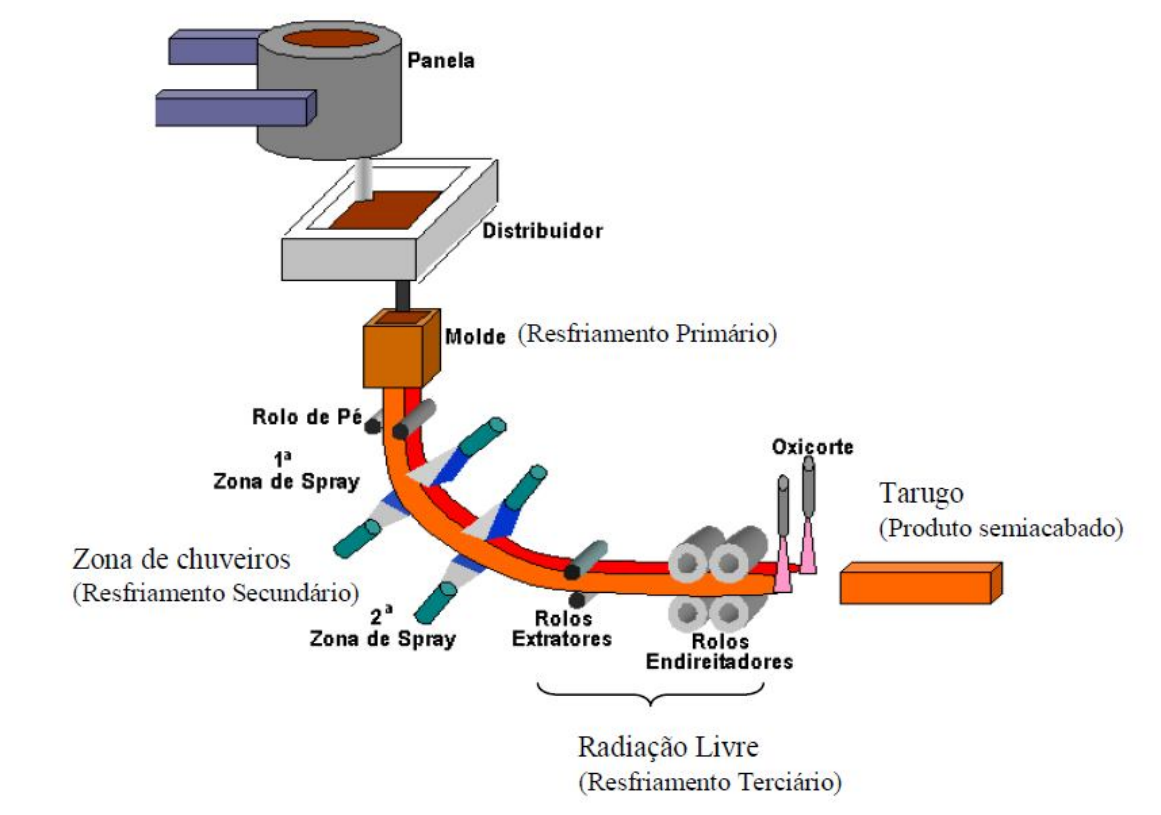
\includegraphics[width=0.8\linewidth]{figuras/Steel/artigo_2.png}
	\caption{Processo de lingotamento Contínuo de Tarugos}
	\legend{Fonte: \citeauthor{freitas2013analise} (\citeyear{freitas2013analise})}
	\label{fig:processLing}
\end{figure}

O processo de lingotamento, na siderúrgica Gerdau, usina de Ouro Branco, consiste no despejamento de uma panela com $\sim~224$ toneladas de aço, a uma temperatura de $\sim~1550~$ºC, no distribuidor que precede o lingotamento (Figura \ref{fig:processLing}).
%
Este processo pode levar de horas a dias sem interrupção.
%
A cada batelada de panela da-se o nome de \textbf{corrida}.


A etapa de solidificação ocorre de fora para dentro do veio\footnote{Veio é o nome que se dá ao conjunto formado pelo molde, a máquina Oxicorte e os rolos de extração e endireitadores. Quanto maior o número de veios, maior a produtividade da máquina, mas mais complexo se torna o seu controle.} em função do contato com as paredes refrigeradas do molde, aspersão de água em \textit{sprays} e perda de calor por radiação para o ambiente. Essa troca de calor faz com que o aço se solidifique gradativamente criando zonas onde o material pode ser encontrado em seus estados sólido na parte exterior do tarugo e líquido no interior.

\begin{figure}[htbp]
	\centering
	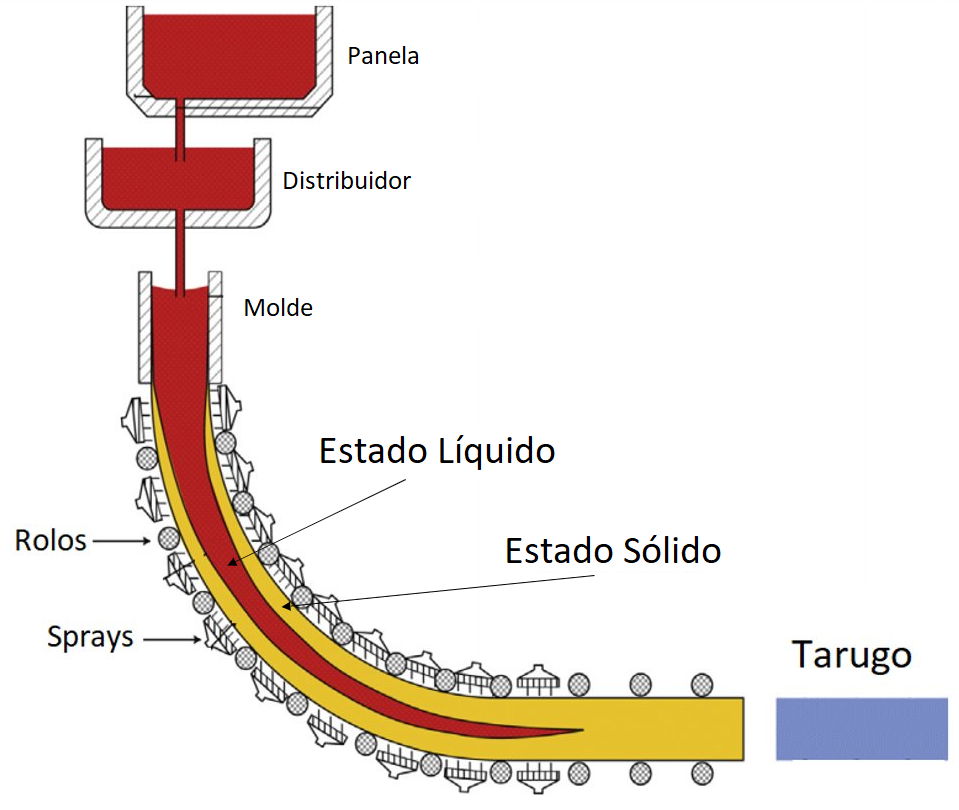
\includegraphics[width=0.8\linewidth]{figuras/Steel/estadoSolidoLiq.png}
	\caption{Estados do aço no processo de lingotamento contínuo}
	\legend{Fonte: \citeauthor{YU201736} (\citeyear{YU201736})}
	\label{fig:processLingSolid}
\end{figure}

No processo final de cada corrida, os tarugos, produto cuja seção transversal é quadrada é usado como matéria prima para laminação,  são cortados na máquina Oxicorte \footnote{Corta o tarugo em um tamanho previamente definido, possibilitando assim o seu trasporte até a sua destinação final.} como mostrado na Figura \ref{fig:processLing}. Os cortes são feitos de acordo com a demanda do cliente e origina em média 100 tarugos, número este que depende do diâmetro das peças que podem ser todas de 130mm ou 160mm e do comprimento das mesmas que variam de 07 a 14m. Após serem cortados, são transportados para o despacho por uma ponte rolante a base de eletroímãs que suportam altas temperaturas e $27$ toneladas de carga. 


\begin{figure}[htbp]
	\centering
	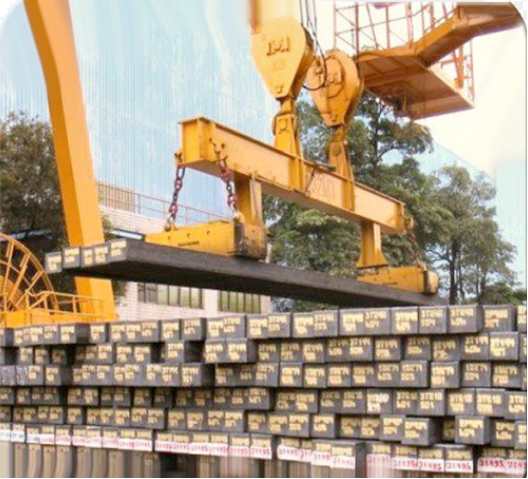
\includegraphics[width=0.7\linewidth]{figuras/Steel/ponte_rolante.png}
	\caption{Ponte Rolante}
	\legend{Fonte: \citeauthor{ponte-rolante} (\citeyear{ponte-rolante})}
	\label{fig:crane}
\end{figure}

\begin{figure}[htbp]
	\centering
	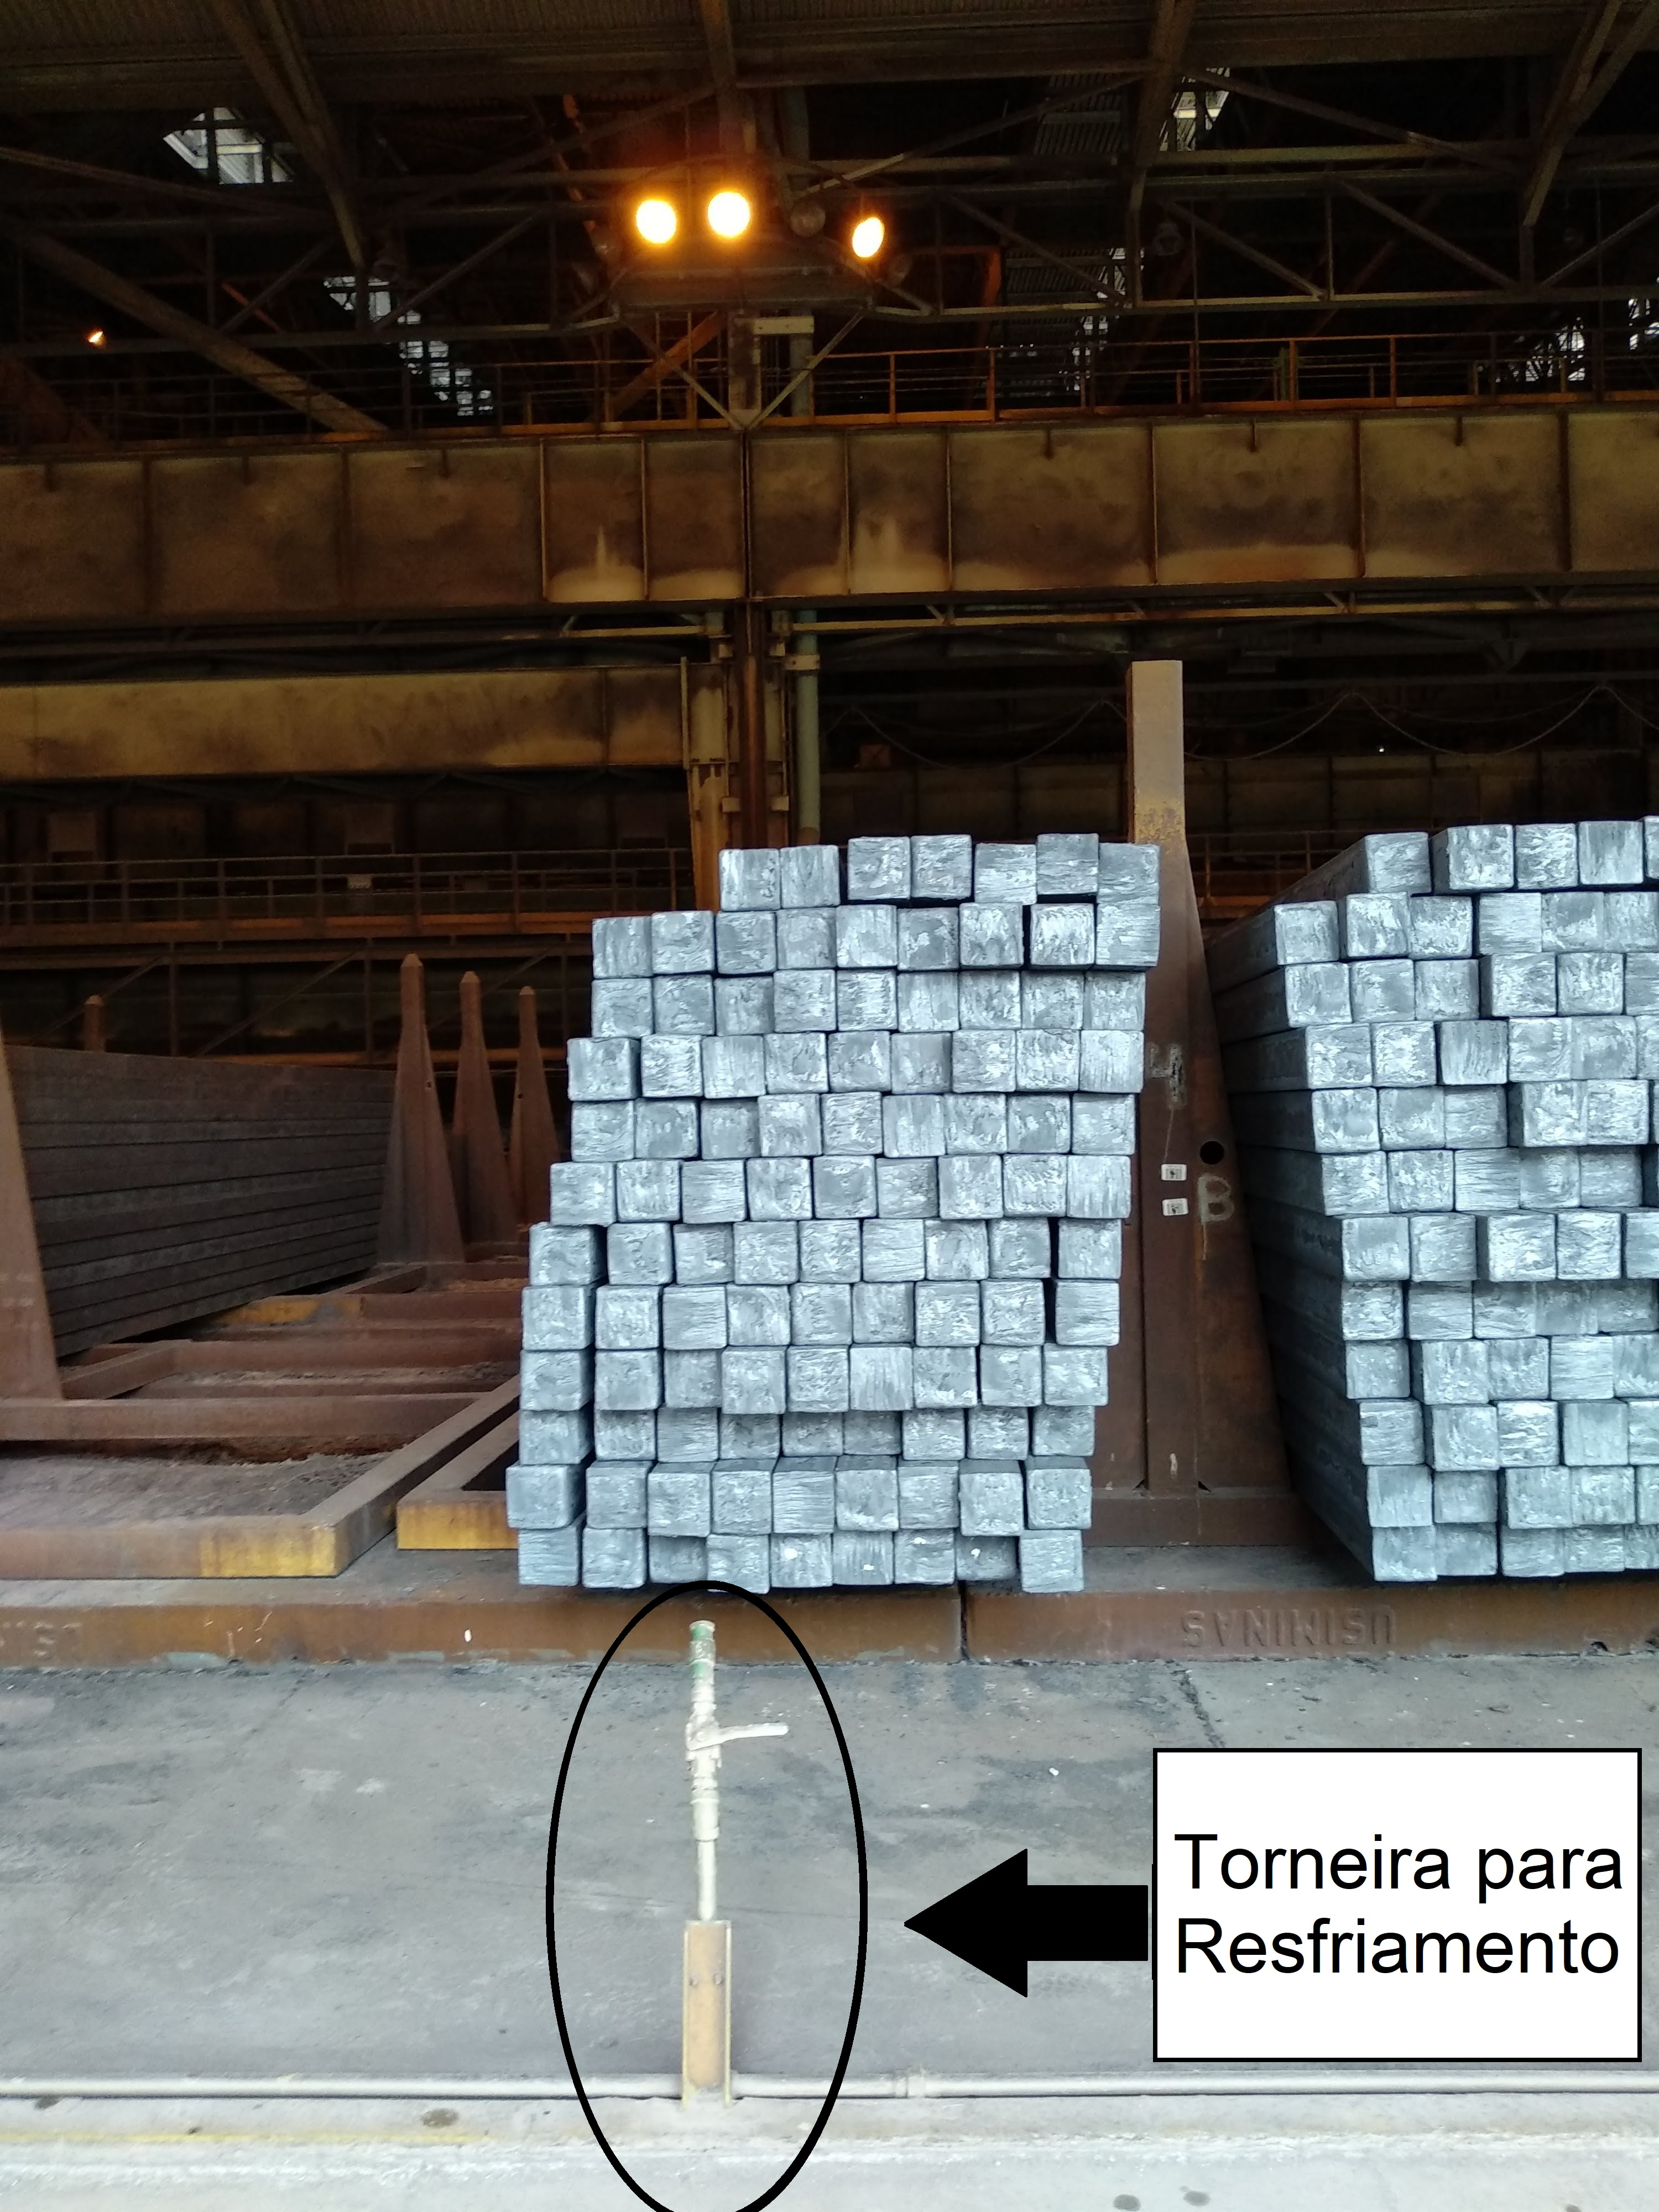
\includegraphics[width=0.5\linewidth]{figuras/Steel/despacho.jpg}
	\caption{Despacho}
	\label{fig:despacho}
\end{figure}

Os tarugos vão para a zona de despacho a uma temperatura de $\sim~700$ºC.
%
Após cerca de 20 horas, a temperatura cai para $150~$ºC, temperatura adequada para a fixação das etiquetas de identificação dos tarugos.
%
Um jato de água é direcionado aos tarugos para acelerar o resfriamento (Figura \ref{fig:despacho}) com frequência constante apenas na parte frontal.
%
A eventual injeção de água no centro do tarugo poderia empenar a peça, uma vez que a temperatura central do tarugo é está mais quente que as extremidades.


Após o tempo necessário, o operador prega as etiquetas utilizando Silicone Acético Transparente, no qual foi testada e comprovada sua eficácia na resistência sobre alta temperatura.

\begin{figure}[htbp]
	\centering
	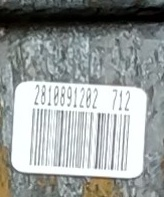
\includegraphics[width=0.25\linewidth]{figuras/Steel/barcode.jpg}
	\caption{Etiqueta}
	\label{fig:barcode}
\end{figure}

A rotulação é importante pois evita a mistura de aço entre uma corrida e outra, viabiliza a rastreabilidade e identificação do aço em processos posteriores como, por exemplo, na laminação até o cliente final. 
%A composição dos números intrinsecos ao códico de barra impresso na etiqueta metálica, como da Figura \ref{fig:barcode}, é o que permite a identificação supracitada a saber:

\begin{table}[]
	\centering
	\begin{tabular}{|l|l|}
		\hline
		\rowcolor[HTML]{ECF4FF} 
		\multicolumn{1}{|c|}{\cellcolor[HTML]{ECF4FF}Número} & \multicolumn{1}{c|}{\cellcolor[HTML]{ECF4FF}2810891202 712}\\ \hline
		28 & Número do convertedor que pode ser CV1 (27) ou CV2 (28).\\ \hline
		108912 & Adicionando o convertedor a este número, forma-se o número da corrida no qual: 
    		    \cr & CV2 = 2 e CV1 = 1, temos
    		    \cr & Número da corrida: 2108912\\ \hline
        02 & 02 é a rota que a panela passou no lingotamento. Ou seja, 02 = tarugo.\\ \hline
        712 & Número 7 é o veio que a peça foi lingotada e 12 o número da peça.\\ \hline
	\end{tabular}
	\caption{Significado dos dígitos da etiqueta de rotulação.}
	\label{tab:tag}
\end{table}

O número de identificação da etiqueta pode ser reconhecido pelos dígitos ou pelo código de barras através de um leitor de código de barras à \textit{laser}. Em cada etiqueta, o código de barras e os dígitos acima deste correspondem à mesma sequência numérica.

Os atuais problemas na identificação das etiquetas são: 
\begin{enumerate}
	\item O processo é atualmente manual e demorado.
	\item O local em que a pilha de peças se encontra é perigoso devido ao fato de, a todo momento, uma ponte rolante estar trabalhando no mesmo local.
\end{enumerate}

% TODO Aqui é o momento ideal pra aparecer uns 2/3 parágrafos de revisão bibliográfica hein kkk Cite dos esforços em automatizar o processo (se houve) e o que outros autores já fizeram em áreas similares. :)

\section{Objetivos} 

Desenvolver um sistema automático para a identificação robusta e geração do relatório de corrida.

Através de uma foto, o sistema será capaz de identificar as etiquetas fixadas no Tarugo, contar o número de etiquetas, identificar o código de barras e, além disso, identificar os números que se encontram acima do mesmo.

Será criado uma aplicação Web com um servidor \textit{online} para que o usuário final possa administrar o sistema através de telas com um \textit{layout} mais amigável.

\subsection{Objetivos específicos}

\begin{itemize}
	\item Recolher várias imagens contendo todos os Tarugos;
	\item Implementar o sistema de expansão dos \textit{datasets} através do método \textit{Data Augmentation}, para que a quantidade de imagens seja suficiente para treinar os modelos de \textit{Machine Learning};
	\item Treinar e implementar o modelo de reconhecimento de código de barras;
	\item Treinar e implementar o modelo de reconhecimento de números;
	\item Implementar a aplicação Web;
	\item Publicar a aplicação no Google Cloud Plataform;
	\item Integrar todos os sistemas a fim de garantir as funcionalidades do projeto;
	\item Executar os procedimentos em ambiente online a fim de validar o projeto;
\end{itemize}

%\section{Justificativas e Relev{\^a}ncia}

\section{Organização do trabalho}

O presente trabalho está organizado em 5 capítulos. No Capítulo 1, encontra-se
a apresentação do problema e suas possíveis soluções, além de apresentar os objetivos
propostos.

O Capítulo 2 consiste nas definições e nas explicações das linguagens de programação, dos métodos e dos \textit{softwares} utilizados no projeto.

No Capítulo 3 é apresentado a estrutura geral do sistema, a metodologia em que foi construído. Explica-se também as etapas do desenvolvimento e códigos implementados.

O Capítulo 4 trata dos experimentos realizados no sistema e seus resultados.

No Capítulo 5 são abordadas as considerações finais do trabalho.